\section{Time-Dependent Schrödinger Equation}

\begin{frame}{Approach to the Schrödinger equation}
    Moving in the quantum realm, our next goal is to approximate the solution of a \textbf{1D time-dependent \textcolor{BrickRed}{Schrödinger equation}}:

    \begin{equation*}
        \fcolorbox{BrickRed}{white}{\text{$\displaystyle i\hbar\frac{\partial\psi}{\partial t}=-\frac{\hbar^2}{2m}\frac{\partial^2\psi}{\partial x^2}+V(x)\psi(x,t)$}}
    \end{equation*}

    \pause

    \begin{equation*}
        \Big\Downarrow
    \end{equation*}

    \small

    \begin{equation*}
        \underbrace{i\hbar\sum_{j=1}^N\frac{d\psi_j}{dt}\int_{-L}^L\phi_j\phi_idx}_{i\hbar M\frac{d\boldsymbol{\psi}}{dt}}=\underbrace{\frac{\hbar^2}{2m}\sum_{j=1}^N\psi_j\int_{-L}^L\frac{\partial\phi_j}{\partial x}\frac{\partial\phi_i}{\partial x}dx}_{\frac{\hbar^2}{2m}A\boldsymbol{\psi}}+\sum_{j=1}^N\psi_j\int_{-L}^LV\phi_j\phi_idx
    \end{equation*}

    \normalsize
\end{frame}

\begin{frame}{Potential matrix}
    In the equation it appears a \underline{linear term}.

    \pause
    
    We must then introduce a new matrix, that can be called \textcolor{BrickRed}{\textbf{potential matrix}}, which is nothing different than a \textbf{weighted mass matrix}:

    \begin{equation*}
        V:V_{i,j}=\int_\Omega V(x)\phi_j(x)\phi_i(x)dx
    \end{equation*}

    \pause

    \begin{equation*}
        \Big\Downarrow
    \end{equation*}

    \begin{equation*}
        i\hbar M\frac{d\boldsymbol{\psi}}{dt}=\frac{\hbar^2}{2m}A\boldsymbol{\psi}+V\boldsymbol{\psi}
    \end{equation*}

    \pause

    \begin{equation*}
        \Big\Downarrow
    \end{equation*}

    \begin{equation*}
        \fcolorbox{BrickRed}{white}{\text{$\displaystyle M\frac{d\boldsymbol{\psi}}{dt}=-\frac{i}{\hbar}\left(\frac{\hbar^2}{2m}A+V\right)\boldsymbol{\psi}$}}
    \end{equation*}
\end{frame}

\begin{frame}{Application of the Cranck-Nicholson method}
    In this case, the PDE is of \underline{first order} in time.

    \pause

    The most suitable method to use is the \textcolor{BrickRed}{\textbf{Crank-Nicholson}} scheme:

    \begin{equation*}
        M\frac{\boldsymbol{\psi}^{(n+1)}-\boldsymbol{\psi}^{(n)}}{\Delta t}=-\frac{i}{2\hbar}\left(\frac{\hbar^2}{2m}A+V\right)\boldsymbol{\psi}^{(n+1)}-\frac{i}{2\hbar}\left(\frac{\hbar^2}{2m}A+V\right)\boldsymbol{\psi}^{(n)}
    \end{equation*}

    \pause

    \begin{equation*}
        \Big\Downarrow
    \end{equation*}

    \begin{equation*}
        \fcolorbox{BrickRed}{white}{\text{$\displaystyle\left[M+\frac{i\Delta t}{2\hbar}\left(\frac{\hbar^2}{2m}A+V\right)\right]\boldsymbol{\psi}^{(n+1)}=\left[M-\frac{i\Delta t}{2\hbar}\left(\frac{\hbar^2}{2m}A+V\right)\right]\boldsymbol{\psi}^{(n)}$}}
    \end{equation*}
\end{frame}

\begin{frame}{How to handle imaginary part}
    The imaginary unit implies that the wavefunction is \underline{complex-valued}.

    \pause

    In order to work with standard real-valued FEM solvers, we apply a \textcolor{BrickRed}{\textbf{real-imaginary splitting}}:

    \begin{equation*}
        \boldsymbol{\psi}^{(i)}=\boldsymbol{u}^{(i)}+i\boldsymbol{w}^{(i)}
    \end{equation*}

    \pause

    Setting $\alpha=\frac{\Delta t}{2\hbar}$ and $H=\frac{\hbar^2}{2m}A+V$:

    \begin{equation*}
        \left(M+i\alpha H\right)\left(\boldsymbol{u}^{(n+1)}+i\boldsymbol{w}^{(n+1)}\right)=\left(M-i\alpha H\right)\left(\boldsymbol{u}^{(n)}+i\boldsymbol{w}^{(n)}\right)
    \end{equation*}

    \pause

    \begin{equation*}
        \Big\Downarrow
    \end{equation*}

    \begin{equation*}
        \begin{cases}
            M\boldsymbol{u}^{(n+1)}-\alpha H\boldsymbol{w}^{(n+1)}=M\boldsymbol{u}^{(n)}+\alpha H\boldsymbol{w}^{(n)}\\
            \alpha H\boldsymbol{u}^{(n+1)}+M\boldsymbol{w}^{(n+1)}=-\alpha H\boldsymbol{u}^{(n)}+M\boldsymbol{w}^{(n)}
        \end{cases}
    \end{equation*}
\end{frame}

\begin{frame}{Block matrix formulation}
    Concatenating real and imaginary components in a \underline{\textit{single} vector}, the final expression is

    \begin{equation*}
        \fcolorbox{BrickRed}{white}{\text{$\displaystyle\begin{pmatrix}
            M & -\alpha H\\
            \alpha H & M
        \end{pmatrix}
        \begin{pmatrix}
            \boldsymbol{u}^{(n+1)}\\
            \boldsymbol{w}^{(n+1)}
        \end{pmatrix}
        =
        \begin{pmatrix}
            M & \alpha H\\
            -\alpha H & M
        \end{pmatrix}
        \begin{pmatrix}
            \boldsymbol{u}^{(n)}\\
            \boldsymbol{w}^{(n)}
        \end{pmatrix}$}}
    \end{equation*}

    \vfill

    \normalsize

    \begin{center}
        As before, the problem is recast as a \textbf{linear system of equations}.
   \end{center}

    \vfill
\end{frame}

\begin{frame}{Free particle scenario}
    If $V(x)=0$, the solution of the Schrödinger equation describes a system called \textcolor{BrickRed}{\textbf{free particle}}.

    \pause

    \vfill

    A \textbf{gaussian} $\mathcal{G}\left(x|x_0,\sigma_0\right)$ can be chosen as \textit{initial wave packet}:

    \begin{equation*}
        \psi(x,0)=\left(\pi\sigma_0^2\right)^{-\frac{1}{4}}e^{-\frac{\left(x-x_0\right)^2}{2\sigma_0^2}+ik_0x}
    \end{equation*}

    We know the analytical solution of the equation:

    \begin{equation*}
        \fcolorbox{BrickRed}{white}{\text{$\displaystyle\psi(x,t)=\frac{1}{\sigma_t\sqrt{\pi}}e^{-\frac{\left(x-x_0-\frac{\hbar k_0}{m}t\right)^2}{\sigma_t^2}} \ \ \ \ \text{where} \ \sigma_t=\sigma_0\sqrt{1+\left(\frac{\hbar t}{m\sigma_0^2}\right)^2}$}}
    \end{equation*}
\end{frame}

\begin{frame}{Numerical simulation}
    Numerical simulation using FEM confirms the theoretical predictions.

    \begin{figure}[H]
        \centering
        \includegraphics[width=\textwidth]{Immagini/plot-schrodinger-free-particle.png}
    \end{figure}
\end{frame}

\begin{frame}{Ballistic spreading}
    The numerical $\sigma$ follows the same \textbf{ballistic behaviour} up until the time when the wavefunction \underline{reaches the boundary}.

    \begin{equation*}
        \sigma(t)\propto\frac{t}{\sigma_0} \ \longrightarrow \ \text{Bigger $\sigma_0$, slower spreading}
    \end{equation*}

    \pause

    \vfill

    \visible<2>{\begin{minipage}{0.31\textwidth}
        \begin{center}
            $\sigma_0=0.10$
        \end{center}
        \vspace{-0.25cm}
        \begin{figure}
            \centering
            \includegraphics[width=\textwidth]{Immagini/plot-sigma-diff-1.png}
        \end{figure}
    \end{minipage}
    \hfill
    \begin{minipage}{0.31\textwidth}
        \begin{center}
            $\sigma_0=0.15$
        \end{center}
        \vspace{-0.25cm}
        \begin{figure}
            \centering
            \includegraphics[width=\textwidth]{Immagini/plot-sigma-diff-1,5.png}
        \end{figure}
    \end{minipage}
    \hfill
    \begin{minipage}{0.31\textwidth}
        \begin{center}
            $\sigma_0=0.20$
        \end{center}
        \vspace{-0.25cm}
        \begin{figure}
            \centering
            \includegraphics[width=\textwidth]{Immagini/plot-sigma-diff-2.png}
        \end{figure}
    \end{minipage}

    \vspace{-0.15cm}

    \begin{figure}[H]
        \centering
        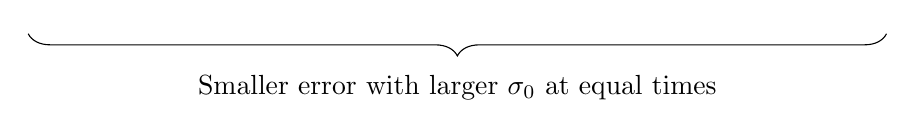
\begin{tikzpicture}
            \draw[decorate, decoration={brace, amplitude=8pt, raise=2pt}] (5.45,0) -- (-5.45,0);

            \node at (0,-0.75) () {Smaller error with larger $\sigma_0$ at equal times};
        \end{tikzpicture}
    \end{figure}}
\end{frame}

\begin{frame}{Periodic potential}
    The introduction of a \textbf{periodic potential} lead to a \textcolor{BrickRed}{\textbf{Kronig-Penney-like model}}, which is used to describe electrons in a crystal lattice.
\end{frame}

\begin{frame}{Conclusions}
    
\end{frame}